\chapter*{Introduction}
\addcontentsline{toc}{chapter}{Introduction}

In recent years, \textit{machine learning} (ML) has been used in many applications, and with all of this success, large datasets have been collected and can be analyzed. For instance, bioinformatics and cheminformatics can gather enormous datasets through high-throughput methods, allowing us to understand genomic data better than ever before. However, these datasets often have many features compared to the number of samples. This often necessitates feature selection before the data is used in a predictive model. A high-performance predictive model with a feature engineering mechanism could bring high value in similar instances.

One such algorithm - REFINED (REpresentation of Features as Images with NEighborhood Dependencies), proposed by \cite{REFINED} converts the high-dimensional data into images and uses a \textit{convolutional neural network} as a predictor. In this work, I explore a streamlined version of this algorithm and compare it to state-of-the-art approaches.

For this approach to make sense, it requires high-dimensional data (an image with a resolution of 3x3 values doesn't make much sense for a CNN). Because of this, I test this approach on data generated using P2Rank by \cite{P2RANK}, which is in the form of a point cloud. The feature vector can be extended by appending the features from the N nearest points. This allows us to create datasets with an arbitrary amount of features. Also, this dataset is from a similar domain to the one used in the original paper, making it the perfect candidate. Lastly, a part of the P2Rank article is also training a ranking model, which allows us to set a baseline for the models.

The simplest way to get an image from a vector is to reshape the vector into a matrix (a black-and-white image in practice). However, this simplest way could be improved by rearranging the pixels into a more advantageous defined order.

The REFINED algorithm's core takes a matrix with randomly distributed features. It creates gradients (i.e., minimizes local contrast) in the image by minimizing the mean difference between adjacent pixels from all data points. This approach is visualized in figure ~\ref{fig:whole-visualisation} and discussed in greater detail in [Tk. add link].

\begin{figure}
    \centering
    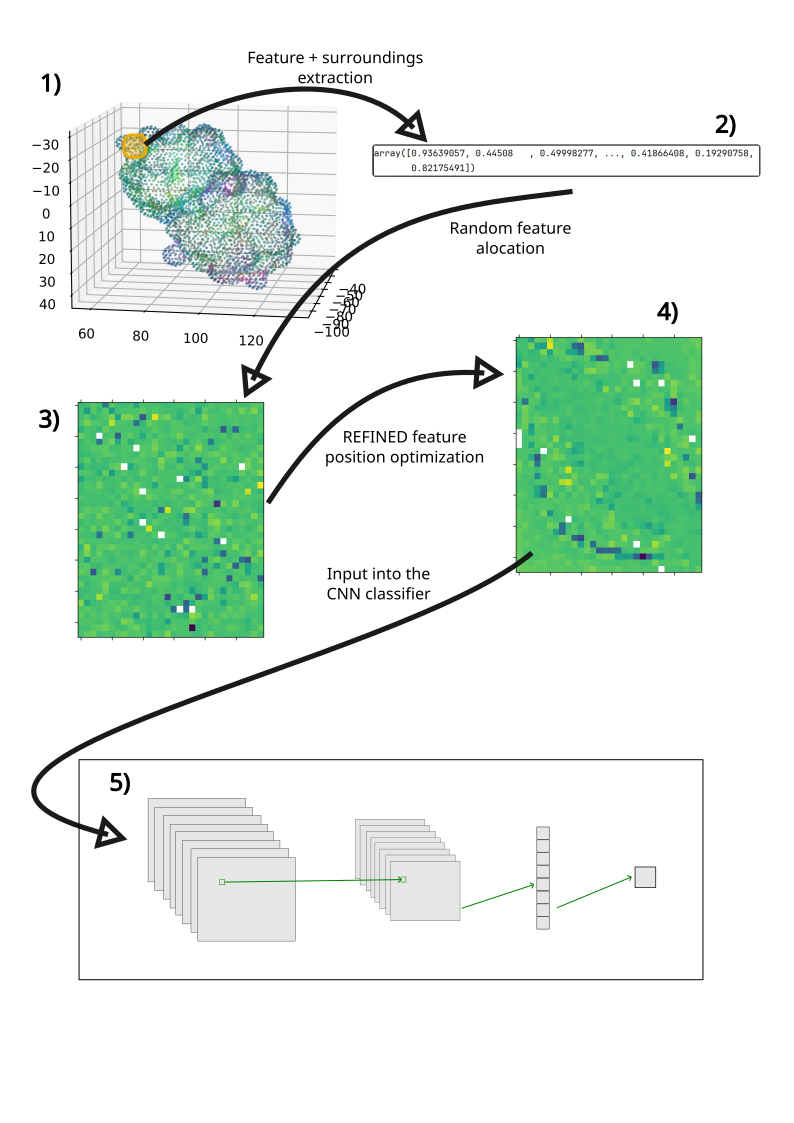
\includegraphics[width=1\linewidth]{whole_pipeline_visualization.png}
    \caption{The general REFINED pipeline. 1) Point cloud, from which features are collected. 2) Long (size $> 900$) feature vector describing a data point. 3) A matrix created by randomly assigning features to positions in the matrix. 4) A REFINED matrix showing gradients created by moving feature positions. 5) CNN model used as a predictor.}
    \label{fig:whole-visualisation}
\end{figure}
